 
% Para una visualizacion correcta, generar el PDF
% Ni el DVI ni el PS se visualizan bien

% Elegir el estilo que se desee, hay cientos en la red

\documentclass{beamer}
\usepackage{beamerthemeshadow}
\usepackage[galician]{babel}
% \usepackage[spanish]{babel}
\usepackage[utf8]{inputenc}
%\usepackage[latin1]{inputenc}

\begin{document}
\title{Título do Traballo de Fin de Grao}
\subtitle{Grao en Enxeñaría Informática \\
Universidade de Santiago de Compostela}  
\author{Autor: Nome do Autor}
\institute{Director: Nome do Director}
\date{\today} 

\begin{frame}
\titlepage
\end{frame}

\begin{frame}
\frametitle{Taboa de contidos}\tableofcontents
\end{frame} 

\section{Sección 1} 
\subsection{Ejemplo de subsección}
\begin{frame}
\frametitle{Título} 
Cada pantalla tiene su título.
\end{frame}

\subsection{Ejemplo de lista}

\begin{frame}
\frametitle{Lista no numerada}
\begin{itemize}
\item una  
\item dos 
\item tres 
\item cuatro
\end{itemize} 
\end{frame}

\begin{frame}
\frametitle{Lista con pausa}
\begin{itemize}
\item número uno \pause 
\item número dos \pause 
\item número tres \pause 
\item número cuatro
\end{itemize} 
\end{frame}

\subsection{Otro ejemplo de lista}
\begin{frame}
\frametitle{Lista numerada}
\begin{enumerate}
\item una  
\item dos 
\item tres 
\item cuatro
\end{enumerate}
\end{frame}

\section{Sección 2} 
\subsection{Tablas}

\begin{frame}
\frametitle{Tablas}
\begin{tabular}{|c|l|r|} \hline
\textbf{Centrado} & \textbf{Izquierda} & \textbf{Derecha} \\ \hline
AAAA  & 1000 & aaaa \\ \hline
BB    & 20   & bb \\ \hline
\end{tabular}
\end{frame}

\begin{frame}
\frametitle{Tabla con pausa}
\begin{tabular}{c c c}
A & B & C \\ \pause 
1 & 2 & 3 \\  \pause 
A & B & C \\ 
\end{tabular} 
\end{frame}

\section{Sección 3}
\subsection{Bloques}

\begin{frame}
\frametitle{Bloques}

\begin{block}{Bloque normal}
Texto del bloque normal
\end{block}

\begin{exampleblock}{Bloque de ejemplo}
Texto del bloque ejemplo
\end{exampleblock}

\begin{alertblock}{Bloque de alerta}
Texto del bloque alerta
\end{alertblock}
\end{frame}

\section{Sección 4}
\subsection{Pantalla dividida}

\begin{frame}
\frametitle{Pantalla dividida}
\begin{columns}
\begin{column}{5cm}
\begin{itemize}
\item una lista
\item de puntos 
\item mas una tabla 
\end{itemize}
\end{column}
\begin{column}{5cm}
\begin{tabular}{|c|c|c|} \hline
\textbf{Mes} & \textbf{Día} & \textbf{Hora} \\ \hline
Enero   & 10 & 15:30 \\ \hline
Febrero & 20 & 20:00 \\ \hline
\end{tabular}
\end{column}
\end{columns}
\end{frame}

\subsection{Figuras} 
\begin{frame}
\frametitle{Incluir figuras}
\begin{figure}

\includegraphics[scale=0.3]{figuras/logo_usc.eps} 
\caption{Logo de la USC}
\end{figure}
\end{frame}

\subsection{Listas con figuras y pausas} 

\begin{frame}
\frametitle{Listas con figuras y pausas}
\begin{columns}
\begin{column}{4cm}
\begin{itemize}
\item<1-> Una
\item<3-> Dos
\item<5-> Tres
\end{itemize}
\vspace{3cm} 
\end{column}
\begin{column}{4cm}
\begin{overprint}
\includegraphics<2>[scale=0.05]{figuras/logo_usc.eps}
\includegraphics<4>[scale=0.10]{figuras/logo_usc.eps}
\includegraphics<6>[scale=0.15]{figuras/logo_usc.eps}
\end{overprint}
\end{column}
\end{columns}
\end{frame}

\subsection{Cuando se necesita más espacio} 
\begin{frame}[plain]
\frametitle{Pantalla plana con sólo una figura}
\begin{figure}
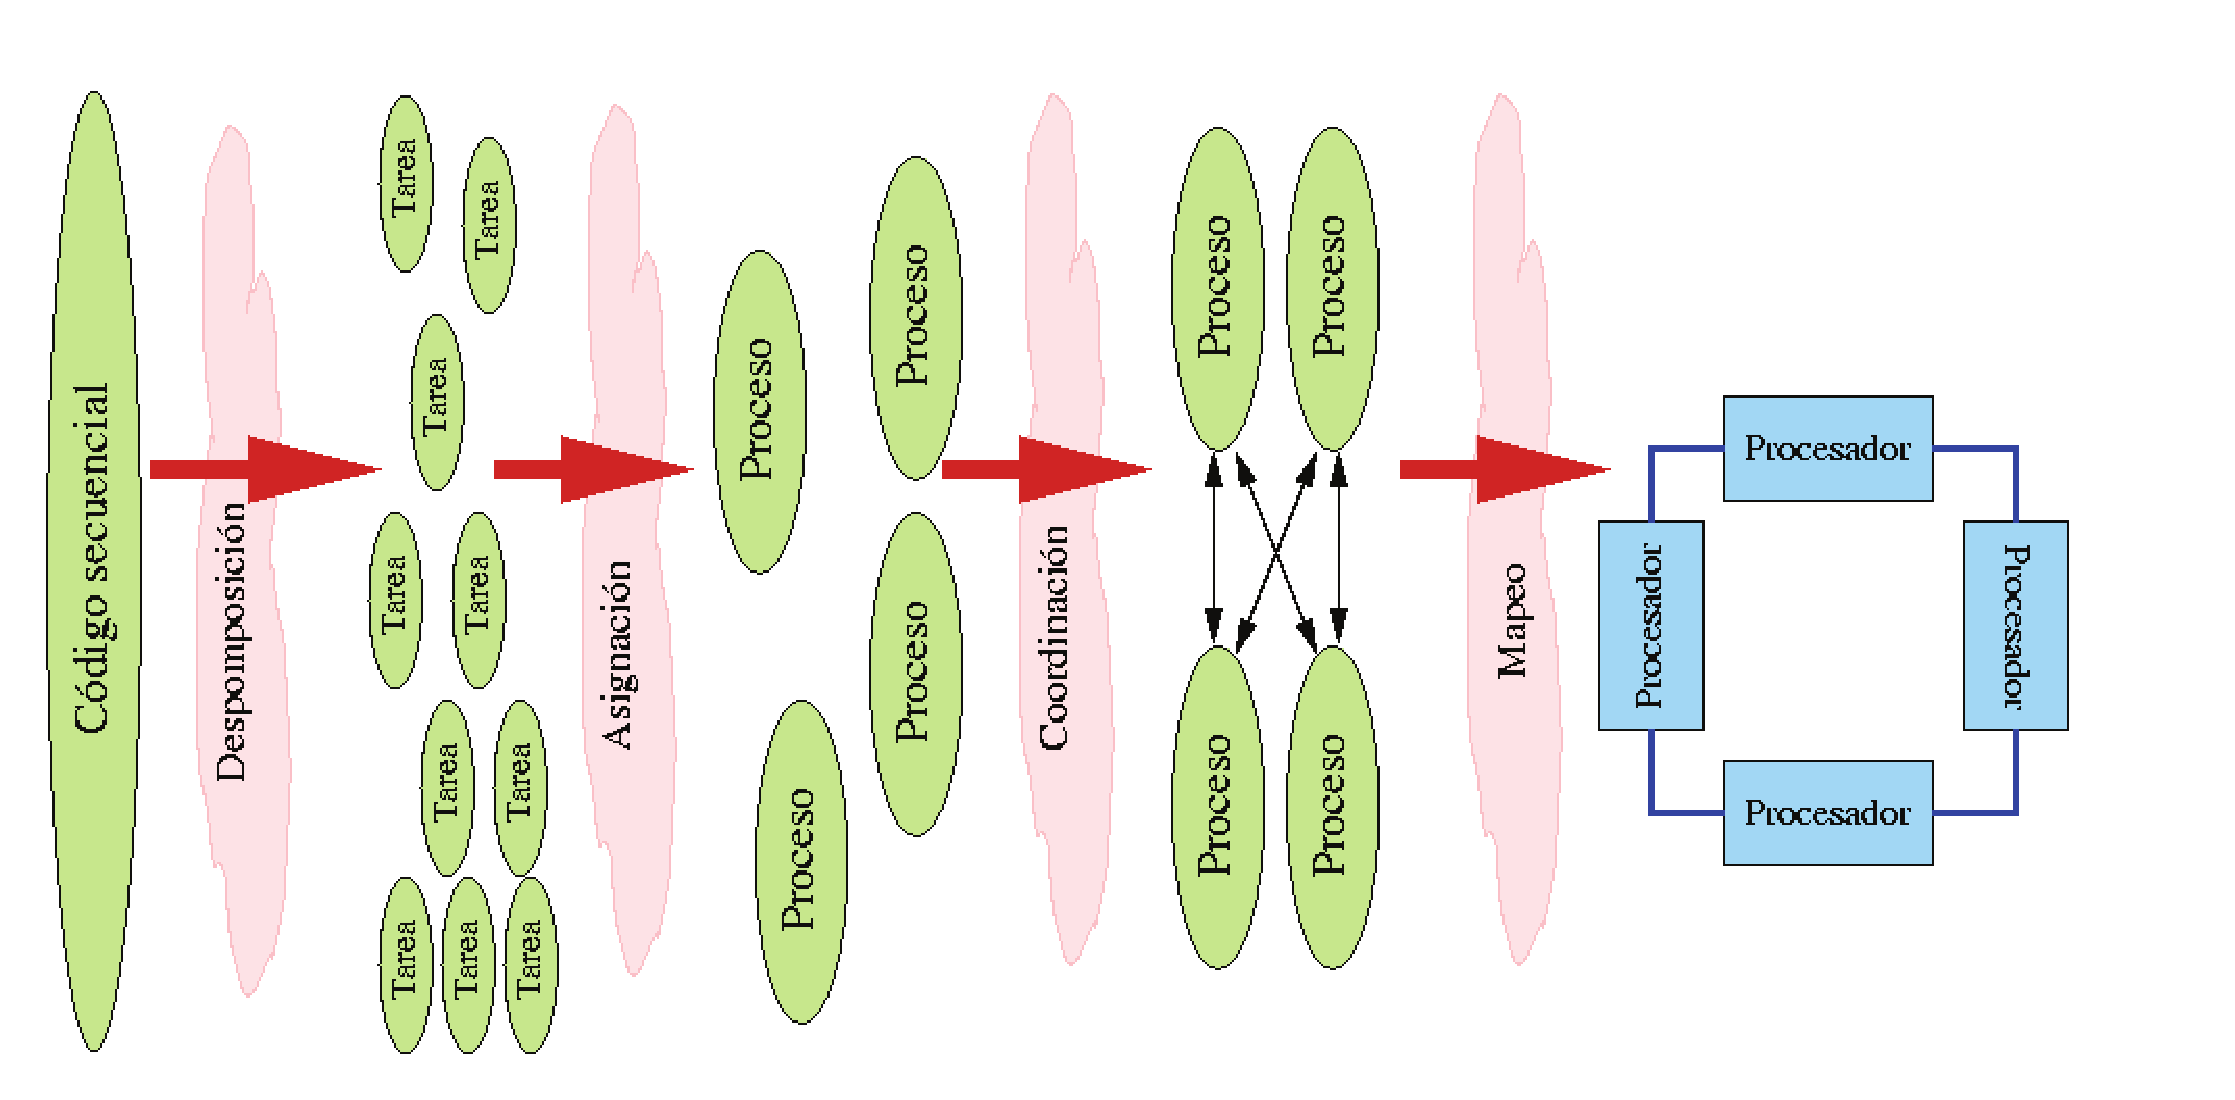
\includegraphics[scale=0.3]{figuras/figura01.eps} 
\caption{Una figura grande}
\end{figure}
\end{frame}

\end{document}

